\documentclass[../../main.tex]{subfiles}
\begin{document}
\begin{oframed}
  \subfile{problem}
\end{oframed}

{\bf [解答]} グラフの概形は\cref{fig:curve_overview}のようになる．

\begin{figure}[htb]
  \centering
  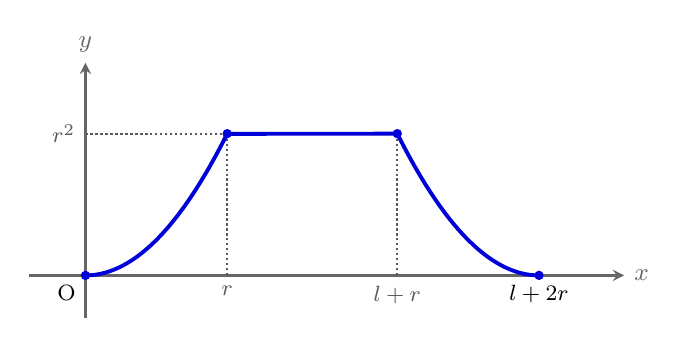
\begin{tikzpicture}[x=1.8cm, y=1.8cm, >=stealth,
    every node/.style={font=\small}]
    \coordinate (O) at (0, 0);
    \coordinate (P1) at (1, 1);
    \coordinate (P2) at (2.2, 1);
    \coordinate (P3) at (3.2, 0);

    % 座標軸
    \draw[->, thick, gray!80!black] (-0.4, 0) -- (3.8, 0) node[right] {$x$};
    \draw[->, thick, gray!80!black] (0, -0.3) -- (0, 1.5) node[above] {$y$};
    \node[below left, font=\footnotesize] at (O) {$\mathrm{O}$};

    % 垂線・射影
    \draw[densely dotted, thick, gray!70!black] (P1) -- (1, 0) node[below, font=\footnotesize] {$r$};
    \draw[densely dotted, thick, gray!70!black] (P1) -- (0, 1) node[left, font=\footnotesize] {$r^2$};
    \draw[densely dotted, thick, gray!70!black] (P2) -- (2.2, 0) node[below, font=\footnotesize] {$l+r$};
    \node[below, font=\footnotesize] at (P3) {$l+2r$};

    % 曲線
    \draw[line width=1.4pt, blue!85!black]
    plot[domain=0:1, samples=60] (\x, {\x*\x})
    -- (P2)
    -- plot[domain=2.2:3.2, samples=60] (\x, {(\x - 3.2)*(\x - 3.2)});

    % 代表点
    \node[circle, fill=blue!85!black, inner sep=1.2pt] at (O) {};
    \node[circle, fill=blue!85!black, inner sep=1.2pt] at (P1) {};
    \node[circle, fill=blue!85!black, inner sep=1.2pt] at (P2) {};
    \node[circle, fill=blue!85!black, inner sep=1.2pt] at (P3) {};
  \end{tikzpicture}
  \caption{曲線の概形}
  \label{fig:curve_overview}
\end{figure}

また，題意の条件から
\begin{align}
  r^2+l=c\label{eq:1}
\end{align}
である．求める体積は，対称性から
\begin{align}
  \dfrac{V}{\pi}=2\int_0^r(x^2)^2\,dx+(r^2)^2l
\end{align}
であるから\cref{eq:1}を代入して
\begin{align}
  \dfrac{V}{\pi}&=2\int_0^rx^4\,dx+r^4(c-r^2)\equiv f(r)
\end{align}
として
\begin{align}
  f'(r)&=2r^4+4cr^3-6r^5 \\
  &=2r^3(-3r^2+r+2c)
\end{align}
である．ただし，$l,r\ge0$から，
\begin{align}
  0\le r^2 \le c \nonumber\\
  0\le r\le \sqrt{c} \label{eq:2}
\end{align}
である．ここで
\begin{align}
  g(r) = -3r^2+r+2c=0 \label{eq:3}
\end{align}
の$2$実解を$\alpha$，$\beta$とする．($\alpha<\beta$)

$g(0)=2c>0$だから，$\alpha<0<\beta$であり，
\begin{align}
  &\beta=\dfrac{1+\sqrt{1+24c}}{6}\le\sqrt{c} \\
  &1+\sqrt{1+24c}\le 6\sqrt{c} \\
  &2+24c+2\sqrt{1+24c}\le 36c \\
  &0\le c(c-1)
\end{align}
に注意して，$c$の値によって場合分けする．

\subparagraph{(i)$1\le c$の時}

増減表は以下のようになる．
\begin{table}[H]
  \centering
  \caption{$1\le c$ のときの $f(r)$ の増減表}
  \label{tab:variation_1_le_c}
  \begin{tabular}{c|c|c|c|c|c}
    $r$ & $0$ & $\dots$ & $\beta$ & $\dots$ & $\sqrt{c}$ \\ \hline
    $f'(r)$ & & $+$ & $0$ & $-$ & \\ \hline
    $f(r)$ & & $\nearrow$ & 極大 & $\searrow$ &
  \end{tabular}
\end{table}

従って，$r=\beta$のとき$V$は最大である．

\subparagraph{(ii)$0<c\le 1$の時}

増減表は以下のようになる．
\begin{table}[H]
  \centering
  \caption{$0<c\le 1$ のときの $f(r)$ の増減表}
  \label{tab:variation_0_lt_c_le_1}
  \begin{tabular}{c|c|c|c}
    $r$ & $0$ & $\dots$ & $\sqrt{c}$ \\ \hline
    $f'(r)$ & & $+$ & \\ \hline
    $f(r)$ & & $\nearrow$ &
  \end{tabular}
\end{table}

故に$r=\sqrt{c}$のとき$V$は最大である．
\casesend

以上および\cref{eq:1}にも注意して，
\begin{align}
  c\ge1&\,\,\,\,
  \begin{cases}
    r=\dfrac{1+\sqrt{1+24c}}{6} \\
    l=\dfrac{6c-1-\sqrt{1+24c}}{18}
  \end{cases}\\
  0<c\le1&\,\,\,\,
  \begin{cases}
    r=\sqrt{c} \\
    l=0
  \end{cases}
\end{align}
のとき$V$は最大である．$\cdots$(答)
\newpage
\end{document}
